\chapter{Background}
\label{chap1b}
This chapter presents a comprehensive overview on the state-of-the-art research on the observation and modelling of pedestrian dynamics, which is the central theme of the thesis. In \cref{chap1b:sec1}, the related literature in data collection methods for pedestrian studies and their transition from traditional questionnaires and surveys, to utilization of modern technologies in recent years are discussed. \cref{chap1b:sec2} reviews the history of pedestrian crossing behaviour and its changes in the context of interacting with automated vehicles. 
\section{Data collection methods in pedestrian studies}
\label{chap1b:sec1}
Any endeavour to understand, model and predict pedestrian dynamics requires the collection of high-quality data on their flow, choices, decisions, preferences, and in general, their behaviour. Traditionally, monitoring and counting pedestrians have been done manually, and by recruiting human resources to observe the pedestrians on site or in the video data. Manual observations have been also a way to understand the Revealed Preferences (RP) of pedestrians. Depending on the objectives of the study, collecting data through surveys, questionnaires and interviews on hypothetical situations has also been a conventional method to understand the Stated Preferences (SP) of pedestrians and their behaviour, or to acquire information about their travel patterns. Each of the aforementioned methods carry their own advantages and disadvantages depending on the purpose of the research that the information is used in. However, all of these traditional methods share some common drawbacks that can negatively affect the quality and size of data if not addressed properly. Traditional methods of data collection are subject to possible human errors as they rely on human resource for data collection and entry~\cite{ryus2014guidebook}. Moreover, relying on human resources for data collection requires workforce recruitment and training, which can be costly, and time-consuming~\cite{lee2017emerging}. In addition, stated preferences experiments are often criticized for the lack of realism when they involve hypothetical scenarios that participants do not have prior exposure to them~\cite{farooq2018virtual}. Systematic bias due to limited number of respondents in SP experiments and interviews is another drawback in traditional approaches in data collections~\cite{wardman1988comparison}. Emergence of novel data sources in the last decade can provide potential solutions to the stated problems. In the next three subsections, an overview of these new data sources is provided in three categories: location-aware technologies for monitoring and detecting pedestrians, virtual reality tools for controlled stated preferences experiments, and open-access automated vehicle datasets for studying pedestrian behaviour from the perspective of the vehicles.       
\subsection{Location-aware technologies}
Using location-aware technologies to automate the data collection has gained popularity among scholars in different fields~\cite{farooq2015ubiquitous}. These modern approaches in data collection have led to a dramatically growing interest in utilizing them in mobility studies as an augmentation or replacement of traditional approaches. Location-aware technologies that have been used for the purpose of detecting, tracking, or counting pedestrians in the relevant research studies include: body-worn sensors, GPS data, GSM network usage data, Wi-Fi Access Point (AP) logs, Bluetooth transceivers data and RFID tags data. In general, these data collection approaches can be divided into two main categories: 1. User-Centric approaches and 2. Network-Centric approaches. \emph{User-Centric} approaches, such as GPS or body-worn sensors, require users to be actively involved in data collection process. Zheng \textit{et al.} used GPS data solely to detect mode of transportation~\cite{zheng2008understanding}. Defining features such as heading change rate, stop rate and velocity change rate and considering the conditional probability between different modes of transport, a graph-based post processing algorithm was proposed to detect network users' mode. To make the results more accurate, some researchers have used multiple data sources simultaneously. Reddy \textit{et al.}, for instance, implemented GPS data along with smartphones accelerometer data to distinguish users movements among walking, running, biking and motorized travelling~\cite{reddy2008determining}. In another study, Stenneth \textit{et al.}, added data from transportation networks to determine user mode of transport among stationery, walking, biking, driving, and using public transit~\cite{stenneth2011transportation}. Although GPS methods provide high accuracy detection, the fact that they necessitate regular users intervention and consume high levels of battery has led scholars to use other, although less accurate, sources. In addition, the need for turning on GPS sensor of the device and installing and running a mobile application to collect GPS records impedes widespread use of these data in real life mobility problems.

 In the \emph{Network-Centric} approach, such as GSM or Wi-Fi on the other hand, data can be collected passively with no intervention from users. Using cellular networks data resolves the problem of battery consumption and users intervention. The basic idea behind user geolocalization with GSM data is to acquire their location based on the identification of the Based Transceiver Stations (BTS) they are connected to in a specific time span. Sohn \textit{et al.}, for example, used coarse grained GSM data to determine whether a user is staying in a place, walking or driving~\cite{sohn2006mobility}.  Wang \textit{et al.} used coarse grained call detail records to infer transportation mode between pairs of defined origins and destinations~\cite{wang2010transportation}. Travellers were clustered into three groups using K-Means algorithm: walking, public transit and driving. Low positioning accuracy, ping-pong handover effect and privacy concerns have been mentioned in this study as some of the main problems of using GSM data. In addition, relatively low density of BTS in some areas make GSM data an unreliable source for detecting mode specially at local levels. For trips within a block or neighborhood, for instance, GSM data cannot be used as a BTS cell size is at least 200 meters~\cite{kalatian2016travel}.
 
 By implementing sensors with the ability to collect connection information from Wi-Fi enabled devices, location and movement data of users can be inferred passively with no intervention from users~\cite{farooq2015ubiquitous}. Wi-Fi enabled devices can be discovered when they are within the coverage range of a Wireless Local Area Network (WLAN), which makes it feasible to extract data from them passively.  Mun \textit{et al.} coupled Wi-Fi and GSM data to train a decision tree classification algorithm for detecting various modes of transportation~\cite{mun2008parsimonious}. Features used for classification in this experiment include: Wi-Fi signal strength Variance, duration of dominant Wi-Fi access point, number of cell IDs that device connects to and residence time in cell footprint. Using Wi-Fi data, tracking indoor movements is also feasible. Various research studies have been conducted for inferring motion in indoor environments. Krumm \textit{et al.}, for instance, used Wi-Fi signal strengths and their variance as inputs to a Hidden Markov Model for smoothing transitions between the inferred states of still and moving~\cite{krumm2004locadio}.
 
 \subsection{Controlled experiments for data collection}
 As a substitution or complementary method to surveys, interviews and stated preferences experiments, controlled experiments can be conducted to assess the pedestrian behaviour under hypothetical scenarios. In some experiments, however, scenarios may be difficult or dangerous to implement in real life. Also, it might be impossible to implement futuristic scenarios involving technologies that are not available to the researchers conducting the experiment. To address these concerns and deliver such scenarios more accurately, pictures, maps and videos have been used in the past~\cite{song2018external}. Recent developments in Virtual Reality (VR) environments have broadened the opportunities for content delivery in a more realistic way~\cite{farooq2018virtual,jennett2008measuring,animesh2011odyssey,nah2011enhancing,faiola2013correlating}. Immersion of users in the VR environment and under controlled condition, allows the evaluation of perceptions, behaviours, choices and preferences of users. Experiments in the VR environments have been conducted successfully in different fields in cognitive studies~\cite{farooq2018virtual}. A user of the VR environment can develop realistic spatial knowledge similar to that of actual physical environments~\cite{o1992effects,ruddle1997navigating}. Physical reactions of users can also be recorded in the VR environments by using electrocardiography, skin conductance or electroencephalogy and eye tracking. In the field of travel behaviour, researchers have used VR in pedestrian route choice studies~\cite{talaat2008simple} and their reaction to information in evacuation scenarios~\cite{kinateder2014virtual}. However, these studies mainly lack the interactive and dynamic potential of VR. More specifically, users in these experiments are only responsible to select routes based on the conditions exposed to them, and are incapable of interacting with other objects in the environment. In order to use the full potential of the VR technology in providing realistic experiments, actions in the VR environment needs to get responses from the elements of the environment, and vice versa. 

One of the main concerns raised in the context of using virtual reality is the level of realism involved and how the results obtained through VR resemble those obtained from behaviours in real life. Several researchers have investigated such comparison. In studies on pedestrian behaviour, Bhagavathula \textit{et al.} compared different elements of pedestrian behaviour in virtual reality and real environments~\cite{bhagavathula2018reality}. Their comparison suggested that the crossing intention, perception of safety, perception of risk and perception of distance were not significantly different in the two environments. On the other hand, it was concluded that the perception of speed in the two approaches of data collection were different among the participants. Similarly, Deb \textit{et al.} compared the behaviour of pedestrians crossing a signalized intersection and concluded that both objective and subjective measures were similar in the participants in the two environments~\cite{deb2017efficacy}. However, an 11\% failure in completing the VR experiments was observed during their data collection, which was a result of motion sickness experienced by the participants. In another study focused on body movements of pedestrians crossing in virtual reality environments, Kalantarov \textit{et al.} concluded that wait time measures in their virtual realty experiment was in line with the laboratory studies and field observations~\cite{kalantarov2018pedestrians}.

\subsection{Open-access AV datasets}
The emergence of automated vehicles has led leading manufacturers and research centers to collect and analyze data using potential AV sensors. Automated vehicles are equipped with several sensors and cameras to detect and explore objects in their surrounding area. Investigating the data and the information that AVs can capture can provide remarkable opportunities for researchers to predict and understand the forthcoming challenges of future urban areas. In this subsection, we review some of the well-known open-access AV datasets. 

Throughout this subsection, we use a number of terms and abbreviations to discuss AV datasets. These terms include:
\begin{itemize}
    \item Ego vehicle: As the operational level of AVs is still limited, some companies and research centers have installed AV sensors on regular vehicles to collect similar to a hypothetical AV. The vehicle that contains the sensors and collects the data is often called the ego vehicle. Some manufacturers use actual AVs as the ego vehicle. 
    \item LIDAR: AVs can be equipped with various sensors. Light Detection and Ranging (LIDAR) is one of the most popular methods in AVs to create a 3D model of the surrounding environment. LIDAR sensors measure distances to the surrounding objects by sending laser pulses to the target and capturing the reflection with a sensor. Using LIDAR sensors as a complementary tool to the video cameras help AVs overcome problems such as occlusion and distortion in video data. 
    \item Annotation: Raw AV datasets contain video and LIDAR data, which often require expert knowledge to process and retrieve useful information. To facilitate the utilization of these data, open-access AV datasets often provide a labelling (manually or automated) of different objects detected in the videos.
\end{itemize}

One of the earliest pioneers of AV datasets is the  Karlsruhe Institute of Technology
and Toyota Technological Institute (KITTI) group. First released in 2012, KITTI dataset is primarily focused on the video data from the cameras installed on an ego vehicle, with GPS and LIDAR data providing the ground truth. With benchmarks provided for different tasks, KITTI is a well-established open-access dataset. However, KITTI is often criticized for a focus on rural areas and highways, and a lack of long enough tracks~\cite{Geiger2013IJRR}. NuScenes is another well-established AV dataset containing 1,000 scenes of 20 seconds length~\cite{nuscenes2019}. Ego vehicles used in nuScenes' data collection contain cameras, LIDAR, RADAR, GPS, and Inertial Measurement Unit (IMU) sensors. Contrary to KITTI, nuScenes includes data from driving in congested urban areas of Boston and Singapore, which makes it a suitable match for studying modern urban spaces. Twenty-three classes of objects are annotated in the dataset, including pedestrians, children, bicycles, construction zones, etc. NuScenes data also include the underlying maps of the drives, which makes it possible to extract some contextual information about the scenes. Although the dataset is collected in different weather conditions, information about the weather is not provided in the dataset and needs to be extracted by processing frames and videos. 
Another dataset built upon nuScenes data format is Lyft Level 5 open data~\cite{lyft2019}. Lyft level 5 dataset provides 2.5 hours of automated driving in Palo Alto, California. Similar to nuScenes, underlying maps, annotations and different weather conditions are included in the dataset. Although it is relatively new, using the same database format as nuScenes gives Lyft level 5 dataset a robust and well-documented structure. The relatively small size of the collected data is the major drawback of Lyft dataset. Ford multi-AV seasonal dataset~\cite{agarwal2020ford} is another relatively new and large dataset concentrated on providing diverse environmental conditions within the data. With a 66 $km$ road coverage over one year of data collection, Ford AV dataset is considered as one of the most extensive datasets regarding its coverage and diversity. However, not providing annotations make this dataset challenging to use in a lot of domains. Google's Waymo dataset is the largest and most annotated AV data currently available ~\cite{sun2020scalability}. With  1,150 scenes of over 6 hours of driving, the covered 76 $km^2$ area in the Waymo dataset is the largest among all the available datasets. Extensive hours of data collection include driving in night time and daylight, construction areas, downtown and suburban areas, and diverse weather conditions.  However, unlike other popular AV datasets, Waymo currently does not provide an underlying map of the drives, making utilization of contextual information from the map impossible.       





 



\section{Interactions of pedestrians and automated vehicles}
\label{chap1b:sec2}
Extensive presence of automated vehicles in urban areas is going to be one of the major changes in near future. In urban areas altered fundamentally by the presence of AVs, studying pedestrians' crossing behaviour is of paramount importance, for the safety of most vulnerable users, optimal roadway layout changes, geometric design updates, and traffic flow optimization. The necessity for new approaches in studying pedestrian and vehicle interactions with an emphasis on investigating mid-block unsignalized crossings raises as AVs, as the rule-obeying agents of future urban space, are expected to always yield to crossing pedestrians~\cite{millard2018pedestrians}. In \cref{fig:frameworkcross}, dynamics of a mid-block unsignalized crossing of a pedestrian is depicted. On the pedestrian's side, waiting on the side walk for a safe gap to initiate a cross, and following a trajectory and its corresponding speed and acceleration to reach the other side of the street are the two behaviours of a crossing pedestrian. Reactions of the vehicle based on the observation of the environment and prediction of pedestrian's behaviours form the vehicle side of the dynamics. The next two sections explore the two parts of the pedestrian side of the these interactions: wait time and trajectory.
\begin{figure}
    \centering
    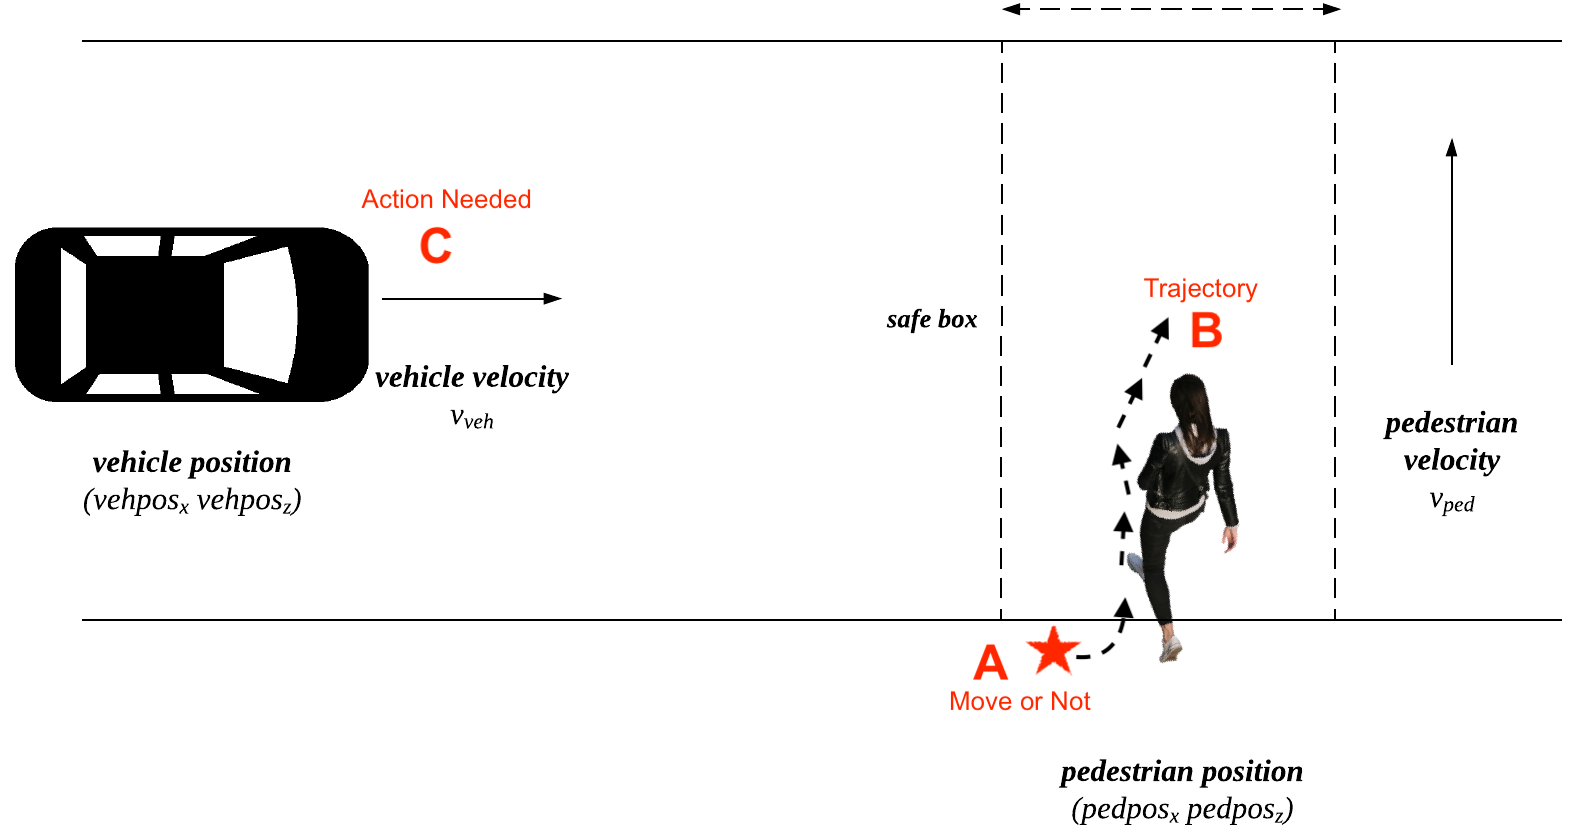
\includegraphics[scale=0.2]{chapter_1b/figures/ped5.png}
    \caption{Vehicles and pedestrians interactions in mid-block crossings}
    \label{fig:frameworkcross}
\end{figure}

\subsection{Pedestrian wait time analysis}
Most studies in pedestrian wait time at unsignalized intersections and mid-block crossings focus on the concept of accepted gap time. Wilson and Grayson~\cite{wilson1980age} analyzed pedestrians' accepting gaps of less than 2 seconds, which is considered to be very short, at a crossing with two-way traffic flow, for different age groups. Results showed that 3.4\% of males and 2\% of females accept these gaps when crossing against nearside traffic. Acceptance rate of such gaps when crossing against far side traffic was higher at 6.2 and 4.8\%, respectively.
On a similar study considering medians, Das~\textit{et al.}~\cite{das2005walk} found that pedestrians waiting on medians accept shorter gaps more easily, compared to those waiting on the curb sides.  According to this study, pedestrians behave more cautiously confronting bigger vehicles. However, the effect of waiting times and number of crossing attempts are not taken into account in this study. In an older study, DiPietro and King~\cite{dipietro1970pedestrian} considered waiting time in their gap time analysis and concluded that by increasing waiting time on the curb, the accepted gaps increases as well. In other words, pedestrians who wait longer before crossing require longer gaps between cars to cross the road. Considering gender of the pedestrians, the results revealed that men were willing to cross using shorter gaps in comparison to women. Moreover this study suggested that, despite having slower pace, pedestrians in group accept shorter gaps than individuals. This finding can be traced back to a couple of reasons, such as the effect of peer pressure to cross, lack of attention, or perception of safety in numbers. Oxley~\textit{et al.}~\cite{oxley2005crossing} focused on the effect of age on the ability to choose safe gap time. By developing a logistic regression model, gap selection was analyzed in their study with respect to walking time, age group, time (or distance) gap and vehicle speed. According to their results, the primary contributing factor in deciding to cross, which can be interpreted as waiting time, appeared to be the distance to upcoming vehicle and time of arrival. Moreover, elderly participants appeared to select more unsafe gap times, given that their walking speeds were slower. In a relatively more recent work, Kadali~\textit{et al.} used Artificial Neural Networks (ANN) to estimate pedestrians' gap acceptance at mid-block unmarked crossings and compared its performance to multiple regression models. Their results showed that ANN has a better prediction performance, being able to consider the effects of higher number of variables. However, the authors mentioned the strength of regression models in such cases due to their ability to reflect the significance of contributing variable. A few researchers have employed game theory models to study pedestrian-vehicle interactions for mid-block unmarked crossings. Sun~\textit{et al.}~\cite{sun2003modeling} for instance, developed a framework for pedestrian-vehicle interaction based on pedestrians’ gap acceptance and motorists yield behaviour. With respect to pedestrians gap acceptance, three types of models were explored: a deterministic model considering gap size, a probabilistic model assuming a certain distribution for gap acceptance as a random variable, and a binary logit model considering age, gender, waiting time, gap size, and number of pedestrians waiting on the curb. Finally, pedestrian and vehicle interactions were modelled as a two-player non-zero-sum non-cooperative game. 

Some studies have tried to model wait time directly, and not through the lens of accepted gap times. In one of the earliest studies of pedestrian crossings at unsignalized crosswalks, Hamed~\cite{hamed2001analysis} used data collected from observations in the city of Amman, Jordan, to investigate the pedestrian waiting time at mid-block locations on divided and undivided roads. A Cox Proportional Hazards (CPH) model was developed to model pedestrian waiting time on the sidewalks. The results suggested that having accident experience, car ownership, number of people on the crosswalk, age, gender, type of trip and vehicle gap time are important factors in determining wait time before crossing. It is interesting to note that the parameters related to traffic were not found to be statistically significant. In another study, Tiwari~\textit{et al.}~\cite{tiwari2007survival}, observed that the average waiting time for females is 27\% more than for males at signalized intersections. In a similar work, Wang~\textit{et al.}~\cite{wang2011individual} developed a parametric survival analysis and found that personal characteristics affect crossing behaviour. In their sample group of study, young men on their way to school were more likely to terminate their waiting time in shorter time. They also indicated that crossing behaviour is highly influenced by safety awareness and conformity behaviour. In another study on modeling pedestrians' waiting time at signalized intersections, Li~\cite{li2013model} applied a statistical modeling approach and proposed a U shaped distribution for pedestrian waiting time at signalized intersections. By developing the model for different age cohorts, it was concluded that the waiting time increases with age.

In a dominant part of the relevant research, survival analysis has proved to be a powerful tool in investigating and understanding the time before an event occurs and the contributing factors in determining that time. In survival analysis, the aim is to estimate time until an event occurs. A collection of statistical modeling methods can be designed for this purpose. The most common methods for survival analysis are the Kaplan-Meier model~\cite{kaplan1958nonparametric} and Cox Proportional Hazard~\cite{cox1972regression} model. The Kaplan-Meier model is a non-parametric model for estimating the survival function in homogeneous groups. This model is very easy to implement, but is unable to account for individuals. To take into account feature vectors and compute survival functions for individuals, Cox Proportional Hazards model is usually the solution. Cox Proportional Hazards model is a semi-parametric model that assumes time component and feature component of hazards function to be proportional. The strength of survival analysis methods in modeling duration times in various fields, particularly in medical research, makes them a suitable approach to analyze wait time.

\subsubsection{Machine learning models for wait time analysis}
Despite being the common method of survival analysis for years, the assumptions made in Cox Proportional Hazards are not always true and have limitations:
\begin{itemize}
    \item It assume a linear combination of features within the hazards function.
    \item It assumes a constant hazards function over time.
\end{itemize}
To address these issues, Chun-Nam Yu~\textit{et al.}~\cite{yu2011learning} introduced the Multi-Task Logistic Regression model. The proposed model in their study can be interpreted as having different time intervals with different logistic regression models estimating the probability of occurrence of an event in that specific time interval. Although Multi-Task Logistic Regression models address some of the problems of the previous methods, they still remain linear, thus they cannot capture the nonlinear complexities within the data. Several researchers, particularly in the field of medical sciences, have tried to address this issue by implementing a deep learning approaches ~\cite{faraggi1995neural,katzman2016deep,luck2017deep}. Faraggi and Simon~ \cite{faraggi1995neural} first incorporated a feed-forward neural network as a shift to nonlinear proportional hazards models. In their model, they replaced the linear combination of features with the output of a neural network with one output node. However, research followed by suggested that their network did not perform better that linear Cox Proportional Hazards models~\cite{mariani1997prognostic}. As the mentioned work were done prior to the outburst of modern deep learning algorithms, Katzman~\textit{et al.}~\cite{katzman2016deep} decided to test the performance of more recent deep networks on survival models. They added fully connected and dropout layers and outperformed the performance of previous linear Cox Proportional Hazards models.

\subsection{Pedestrian movement modeling}
Modeling pedestrian movements is of vital importance in designing sidewalks and venues, planning events, evacuation scenarios, or in from the perspective of an automated vehicle, to predict the next locations of pedestrians. However, due to the inherent irregularity in pedestrians movements~ \cite{bierlaire2003behavioral}, modeling pedestrians may seem more difficult than that of vehicles. In addition, data collection seems to be a bigger problem when it comes to pedestrians, due to the chaotic movements, larger datasets required and pedestrians not necessarily following predefined routes~\cite{danalet2014bayesian}. To capture these chaotic movements, the general solution would be to simplify pedestrian movement decisions by applying models in different levels. In general, pedestrian dynamics can be categorized into three levels, as depicted in \cref{fig:model levels}~\cite{sahaleh2012scenario}. To focus on trajectory of the pedestrians in the presence of the automated vehicles, this section is limited to the operational level, with modeling scenarios where pedestrians are not concerned with the routes, and strategic-level information being inputs as known variables.
\begin{figure}
    \centering
    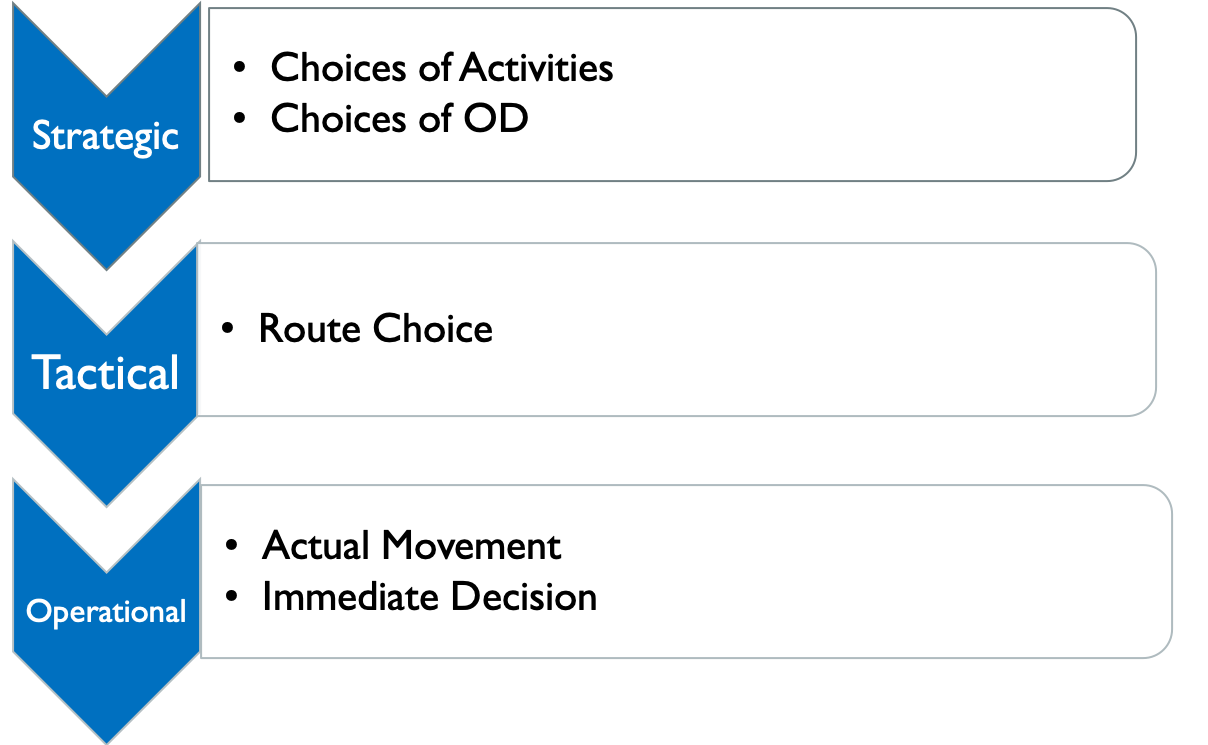
\includegraphics[scale=0.6]{chapter_1b/figures/ped-levels.png}
    \caption{Levels of behaviours for pedestrian movement modeling}
    \label{fig:model levels}
\end{figure}
In general, traditional pedestrian trajectory and movement models can be divided into two main groups: 1) Macroscopic models and 2) Microscopic models. In microscopic models, pedestrians are treated as agents, and are simulated individually. The main drawback of these type of models is the necessity of large and accurate data being available, as individual pedestrian movements require detailed information, based on different parameters. On the other side, macroscopic models consider pedestrians only in groups~\cite{sahaleh2012scenario}. The output for this type of models will then be analyzed based on fundamental diagrams. A diagram of the models discussed in this section can be observed in \cref{fig:tradtypes}, With the dark blue circles representing microscopic models, and macroscopic models represented by light blue filled circles.
\begin{figure}
    \centering
    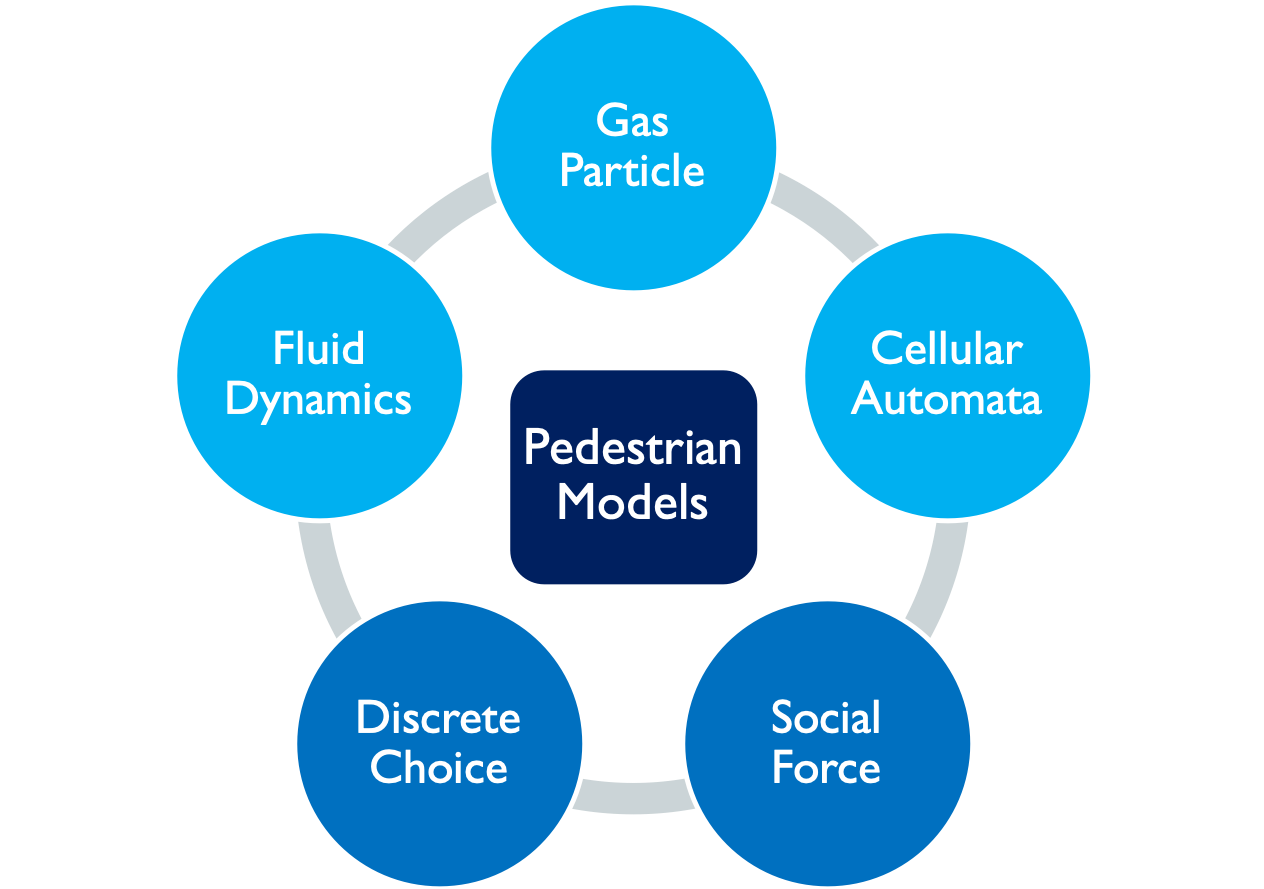
\includegraphics[scale=0.5]{chapter_1b/figures/models.png}
    \caption{Traditional pedestrian trajectory models}
    \label{fig:tradtypes}
\end{figure}
\subsubsection{Gas Particle Models}
Introduced by Henderson in 1974~\cite{henderson1974fluid}, gas particle model assumes movements of pedestrians similar to that of ideal gases. The validation of this model was done by observing data from homogeneous groups of pedestrians, i.e. pedestrians with similar gender, age, walking purpose, etc. that resemble ideal gases. In addition, such models are limited to cases where the density is high. All in all, the idea that human velocity distributions fit the Maxwell-Boltzmann distribution for the velocities of ideal gases for a given temperature, was the start of pedestrian movement modeling, and works properly if the necessary conditions are met.

\subsubsection{Fluid Dynamic Models}
Helbing~\cite{helbing1998fluid} later added some modifications to Gas particle models to account for some microscopic pedestrian phenomena, i.e. interactions between pedestrians, desire to reach a certain density, direction, exit and entrance to the system, and pedestrians reaction times. By adding the above mentioned items, a major step was taken in simulating pedestrian behaviour. Lanes of opposing flows, pedestrian jams and collisions can be observed in visualization of such models. However, low performance of the model in less congested conditions remained a problem.

\subsubsection{Cellular Automata Models}
Another popular macroscopic models for pedestrian movement modeling are cellular automated models ~\cite{blue2001cellular}. The basic concept behind this type of model is to divide the area under study into zones, called cells, and by defining some rules, pedestrians decide their movements between these zones. The first models in this category were defined by simple rules, started from Blue and Adler in 2001~\cite{blue2001cellular}, however later model incorporated more advanced probabilities for moving between cells~\cite{yamamoto2007simulation,weifeng2003simulation}.	
To apply a cellular automated model: The corridor first needs to be divided into similar square cells, with the area  \(\Delta L^2\). In each cell, pedestrians will be homogeneously distributed. To determine the route that the pedestrians choose, possible sequence of areas(contiguous sets of cells) are selected. By grouping pedestrians based on their departure times, size, route, total population in a cell is calculated as the total population of different groups within that cell in each time interval. The flow in each cell can then be calculated as: 
\begin{equation}
    \Delta Q=M.F(M/A)
\end{equation}
 in which $M$ is the population of the cell in the time interval understudy, $A$ is the area of the cell, and $F$ represents the speed-density relationship. 
 
\subsubsection{Discrete Choice Models}
In 2004, Antoninit started applying discrete choice models to pedestrian movement analysis using video recorded data~\cite{antonini2004simulation}. The microscopic approach of the model allowed detailed analysis of movements of people. The choices that the pedestrians are facing at each time in Antoninit's model are speed and direction. Utility functions for each of these choices were defined based on attributes such as presence of obstacles, proximity to the destination and positions and speed of other pedestrians. Later works on these models added other variables, helping the model gain strength by the availability of observing various factors. For instance, Guo \textit{et al.}~\cite{guo2012route} added visibility parameters to the model and Asano \textit{et al.}~\cite{asano2010microscopic} later incorporated density. The major drawback of logit-based microscopic methods is 1. their myopic nature, as they only predict the next step of a pedestrian movement without considering the big picture in terms of steps before and upcoming obstacles and 2. their requirement to discretize the space and speed into arbitrary levels.

\subsubsection{Social Force Models}
Social force model for pedestrians’ dynamics was first introduced by Helbing and Molnar in 1995~\cite{helbing1995social}, based on Lewin’s idea~\cite{lewin1951field} that behavioural changes are caused by so-called social fields. Implementing the idea on pedestrians, Helbing and Molnar described forces affecting pedestrians’ behaviours as a result of internal motivations of an individual to decide and perform actions. They categorized forces on pedestrians in three essential groups:
\begin{itemize}
    \item Forces created by acceleration to reach a desired speed,
    \item Forces that make pedestrians keep a distance to other pedestrians and objects
    \item Forces that represent attractive elements on a pedestrian walk
\end{itemize}

\subsubsection{Machine learning models for pedestrian trajectory}
Widespread success of machine learning methods in recent years, as well as the availability of large pedestrian datasets, have resulted in a shift of research trends to data-driven approaches in pedestrian studies. In one of the major earlier studies in the field, Alahi~\textit{et al.} introduced Social LSTM~\cite{alahi2016social}, a method that incorporated interactions among pedestrians in sequential models, namely Long Short-Term Memory (LSTM), to forecast trajectory of pedestrians using video footage of walking individuals in crowded scenes. In spite of the success of social LSTM model in forecasting pedestrian's trajectory, this model does not account for the contextual information on the environment and aspects like where the pedestrian is looking, thus making it difficult to apply to situations like road crossing behaviours of pedestrians in an automated environment. Furthermore, the future trajectory predicted by Social LSTM assumes a fixed length future trajectory. Lee~\textit{et al.} added semantic context to their proposed RNN model, \textit{DESIRE}~\cite{lee2017desire}, and predicted pedestrian trajectory of variable lengths in video data. More recently, Alahi~\textit{et al.} introduced \textit{Social GANs}~\cite{gupta2018social}, a model that predicts socially acceptable trajectories by training adversarial against a recurrent discriminator. 

\section{Summary}
A new approach to research on pedestrian behaviour requires modern tools on different dimensions. With the availability of big data and powerful methodological frameworks, problems of modern and future urban areas needs to be carefully defined and addressed.  In the era of big data, machine learning and neural networks are becoming an important aspect of understanding and predicting the effects of disruptive mobility on urban roads, as they offer more flexibility and computational efficiencies in handling complex data structures.

The main hypothesis of this dissertation is that by incorporating new data sources and developing novel data-driven models, communities can anticipate, and be well-aware of the changes that have started to happen in urban areas. By taking a pedestrian-oriented point of view, this dissertation seeks to provide policies and recommendations to prepare the cities for these changes, and help the dynamics of urban areas grow in a pedestrian-friendly way. 
This chapter outlined the background theory and existing research in the context of this thesis.
In the next two chapters, passively collected Wi-Fi data and Virtual Reality data are introduced and analyzed as alternative sources of data to track and count, understand and model pedestrian behaviour. \cref{chap4} and \cref{chap6} then use virtual reality data to understand pedestrian crossing behaviour in a futuristic context and in the presence of automated vehicles. Advance neural network modeling frameworks are proposed in these two chapters to replace and improve traditional models. The \textit{black box} nature of neural networks are one of the major obstacles towards a full transition to data-driven machine learning models in transportation research. To account for this concern, machine learning interpretability models are widely discussed and incorporated in this dissertation.

